\renewcommand{\thefigure}{S\arabic{figure}}\renewcommand{\theHfigure}{supp.\arabic{figure}}\setcounter{figure}{0}
\renewcommand{\thetable}{S\arabic{table}}\renewcommand{\theHtable}{supp.\arabic{table}}\setcounter{table}{0}
\clearpage
\begin{figure}[p]
\centering
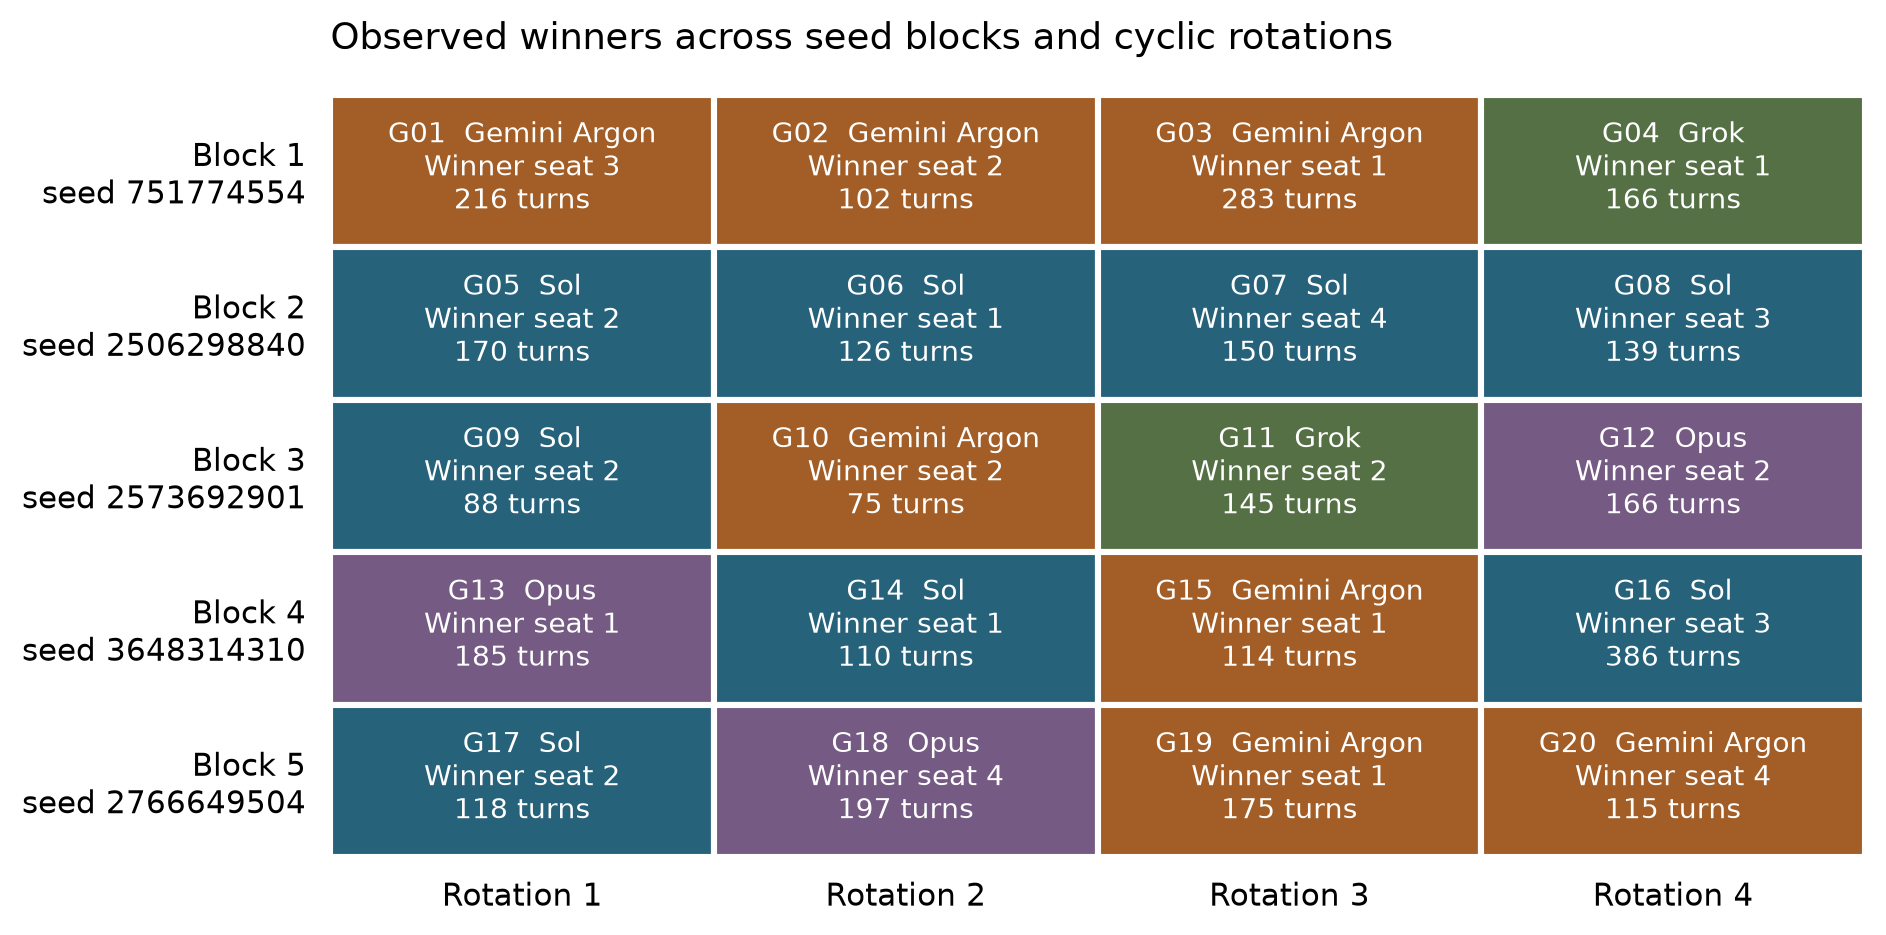
\includegraphics[width=\linewidth,height=0.73\textheight,keepaspectratio]{s1_seed_rotation.png}
\caption[Alternative seed/rotation grid]{Sol's alternative rendering of the same 20 outcomes, not an independent dataset. Seats are one-based. Raster export retained to avoid SVG font-substitution artifacts.}
\label{fig:peer-s1_seed_rotation}
\end{figure}
\clearpage
\clearpage
\begin{landscape}
\begin{figure}[p]
\centering
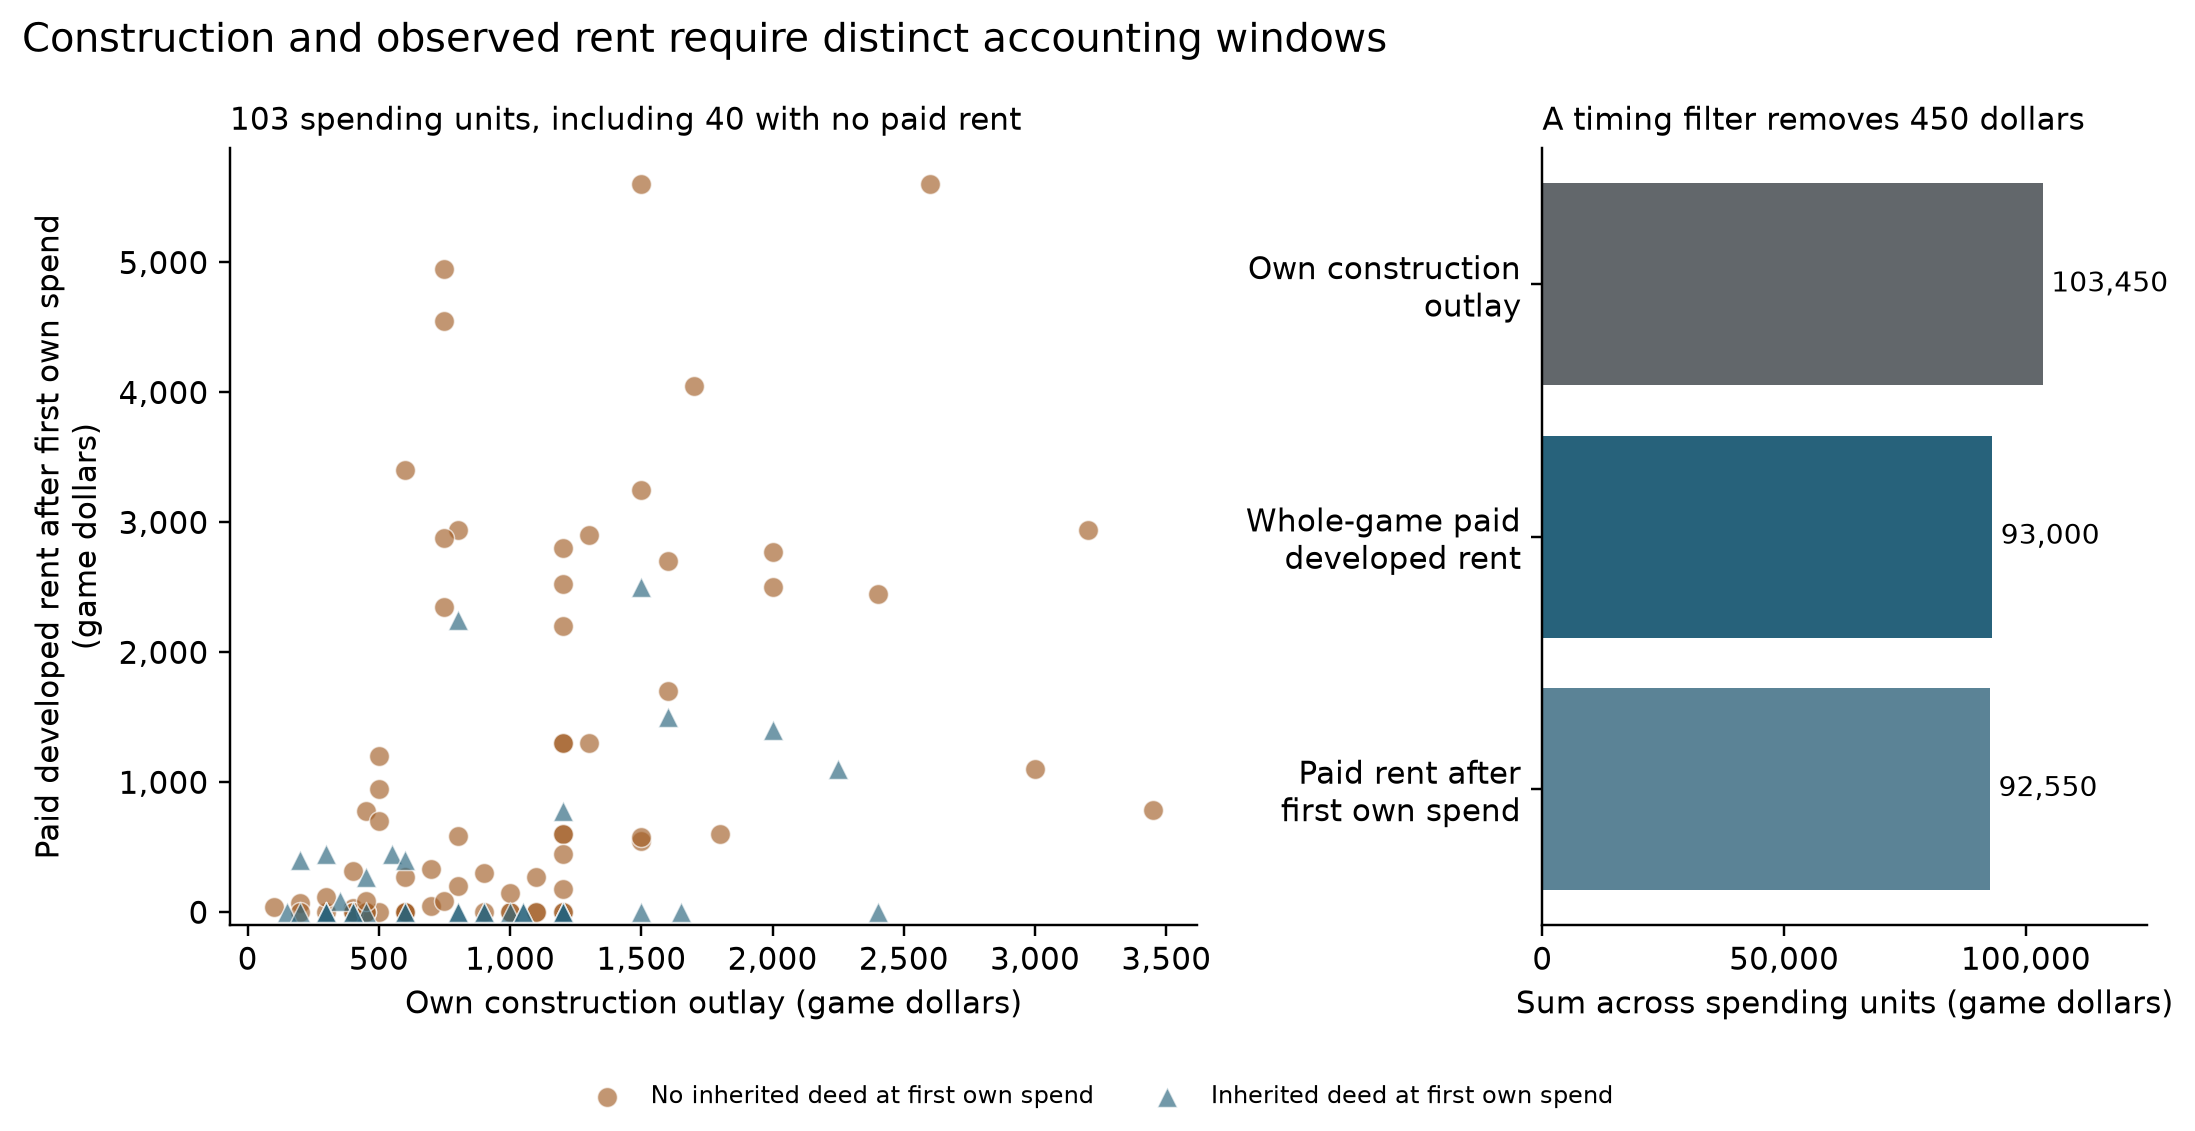
\includegraphics[width=\linewidth,height=4.4in,keepaspectratio]{s2_spending_windows.png}
\caption[Whole-game and post-own-spending receipts]{Sol's two-window comparison for all 103 spending units. Whole-game paid developed rent is 93,000 game dollars; post-own-expenditure receipts are 92,550. No ROI or causal return is identified. Raster export.}
\label{fig:peer-s2_spending_windows}
\end{figure}
\clearpage
\end{landscape}
\clearpage
\begin{figure}[p]
\centering
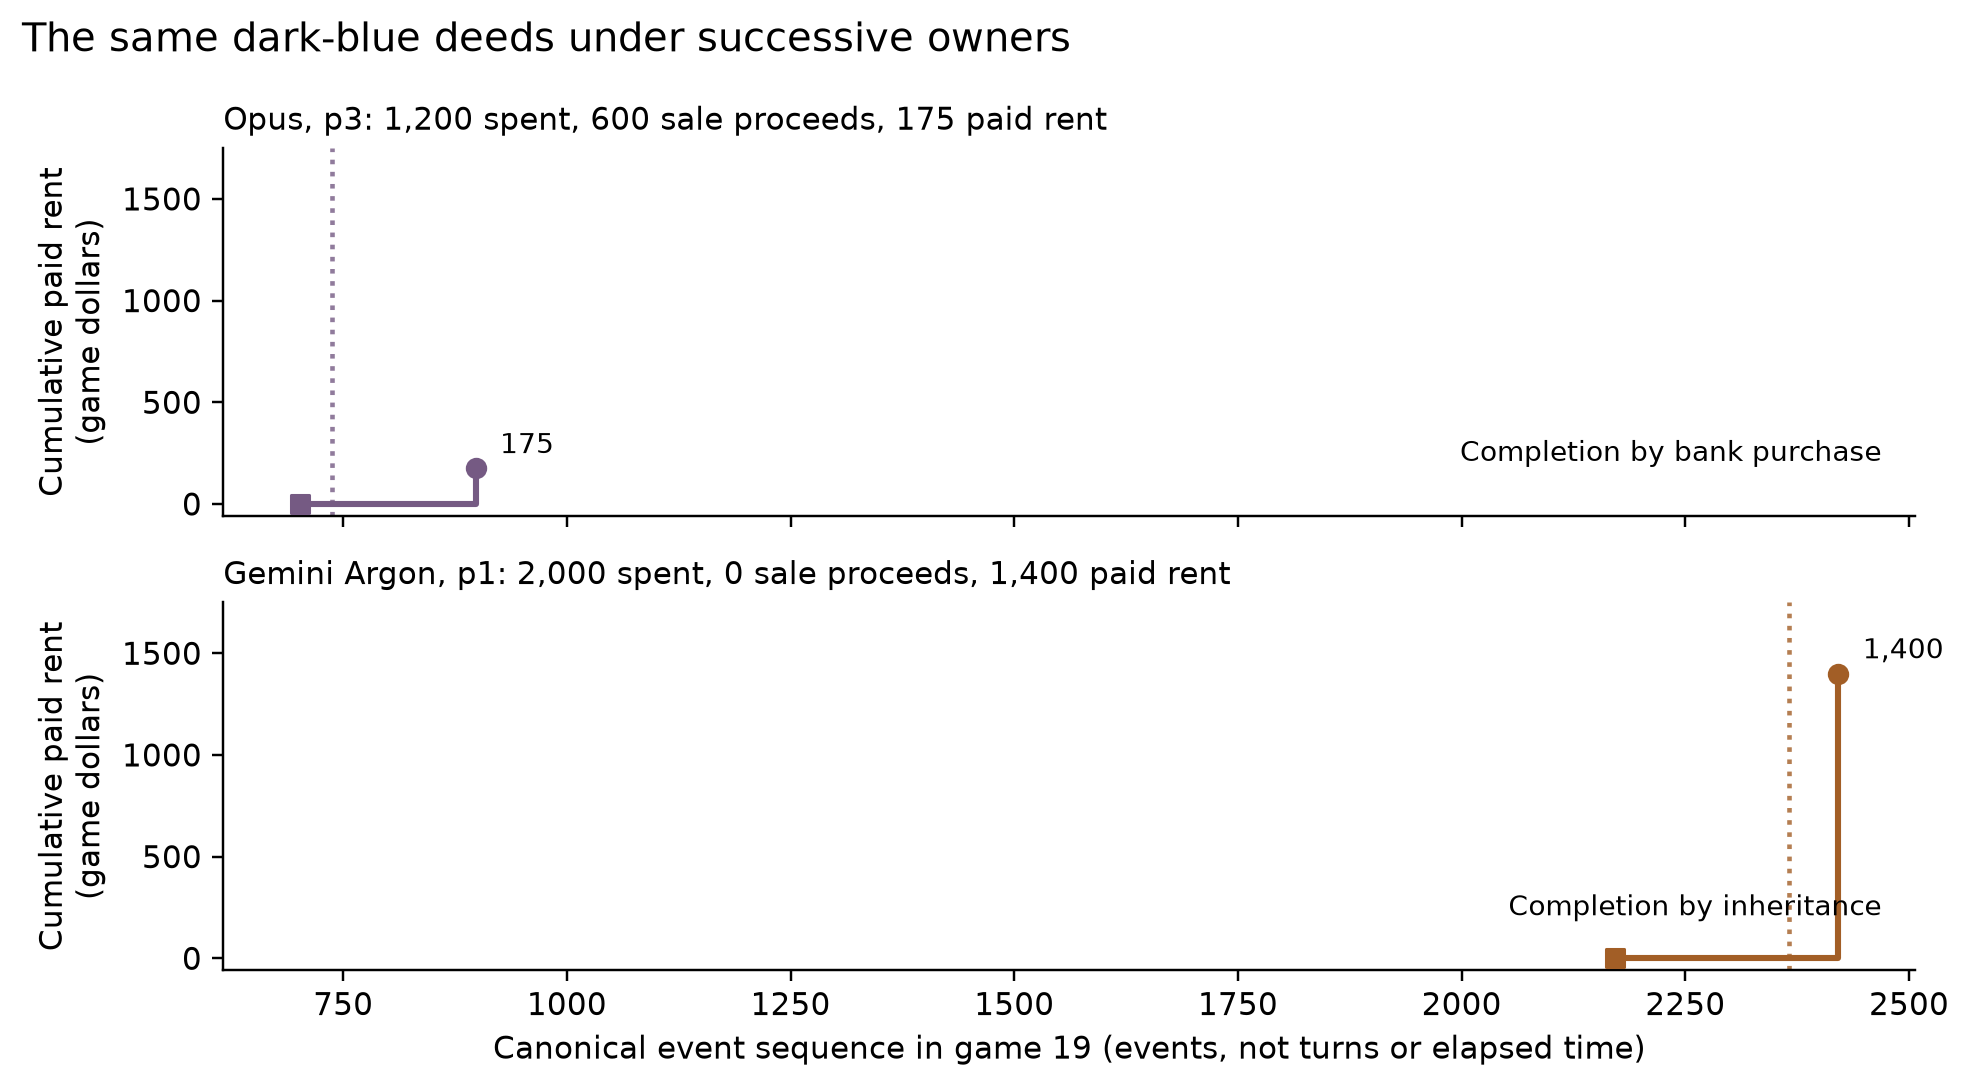
\includegraphics[width=\linewidth,height=0.73\textheight,keepaspectratio]{s3_g19_dark_blue.png}
\caption[G19 dark blue across successive owners]{Sol's event-linked ownership, spending and receipts chronology. The same group has different owners and expenditure histories; whole-game receipts cannot be assigned automatically to an owner's own construction. Raster export.}
\label{fig:peer-s3_g19_dark_blue}
\end{figure}
\clearpage
\clearpage
\begin{figure}[p]
\centering
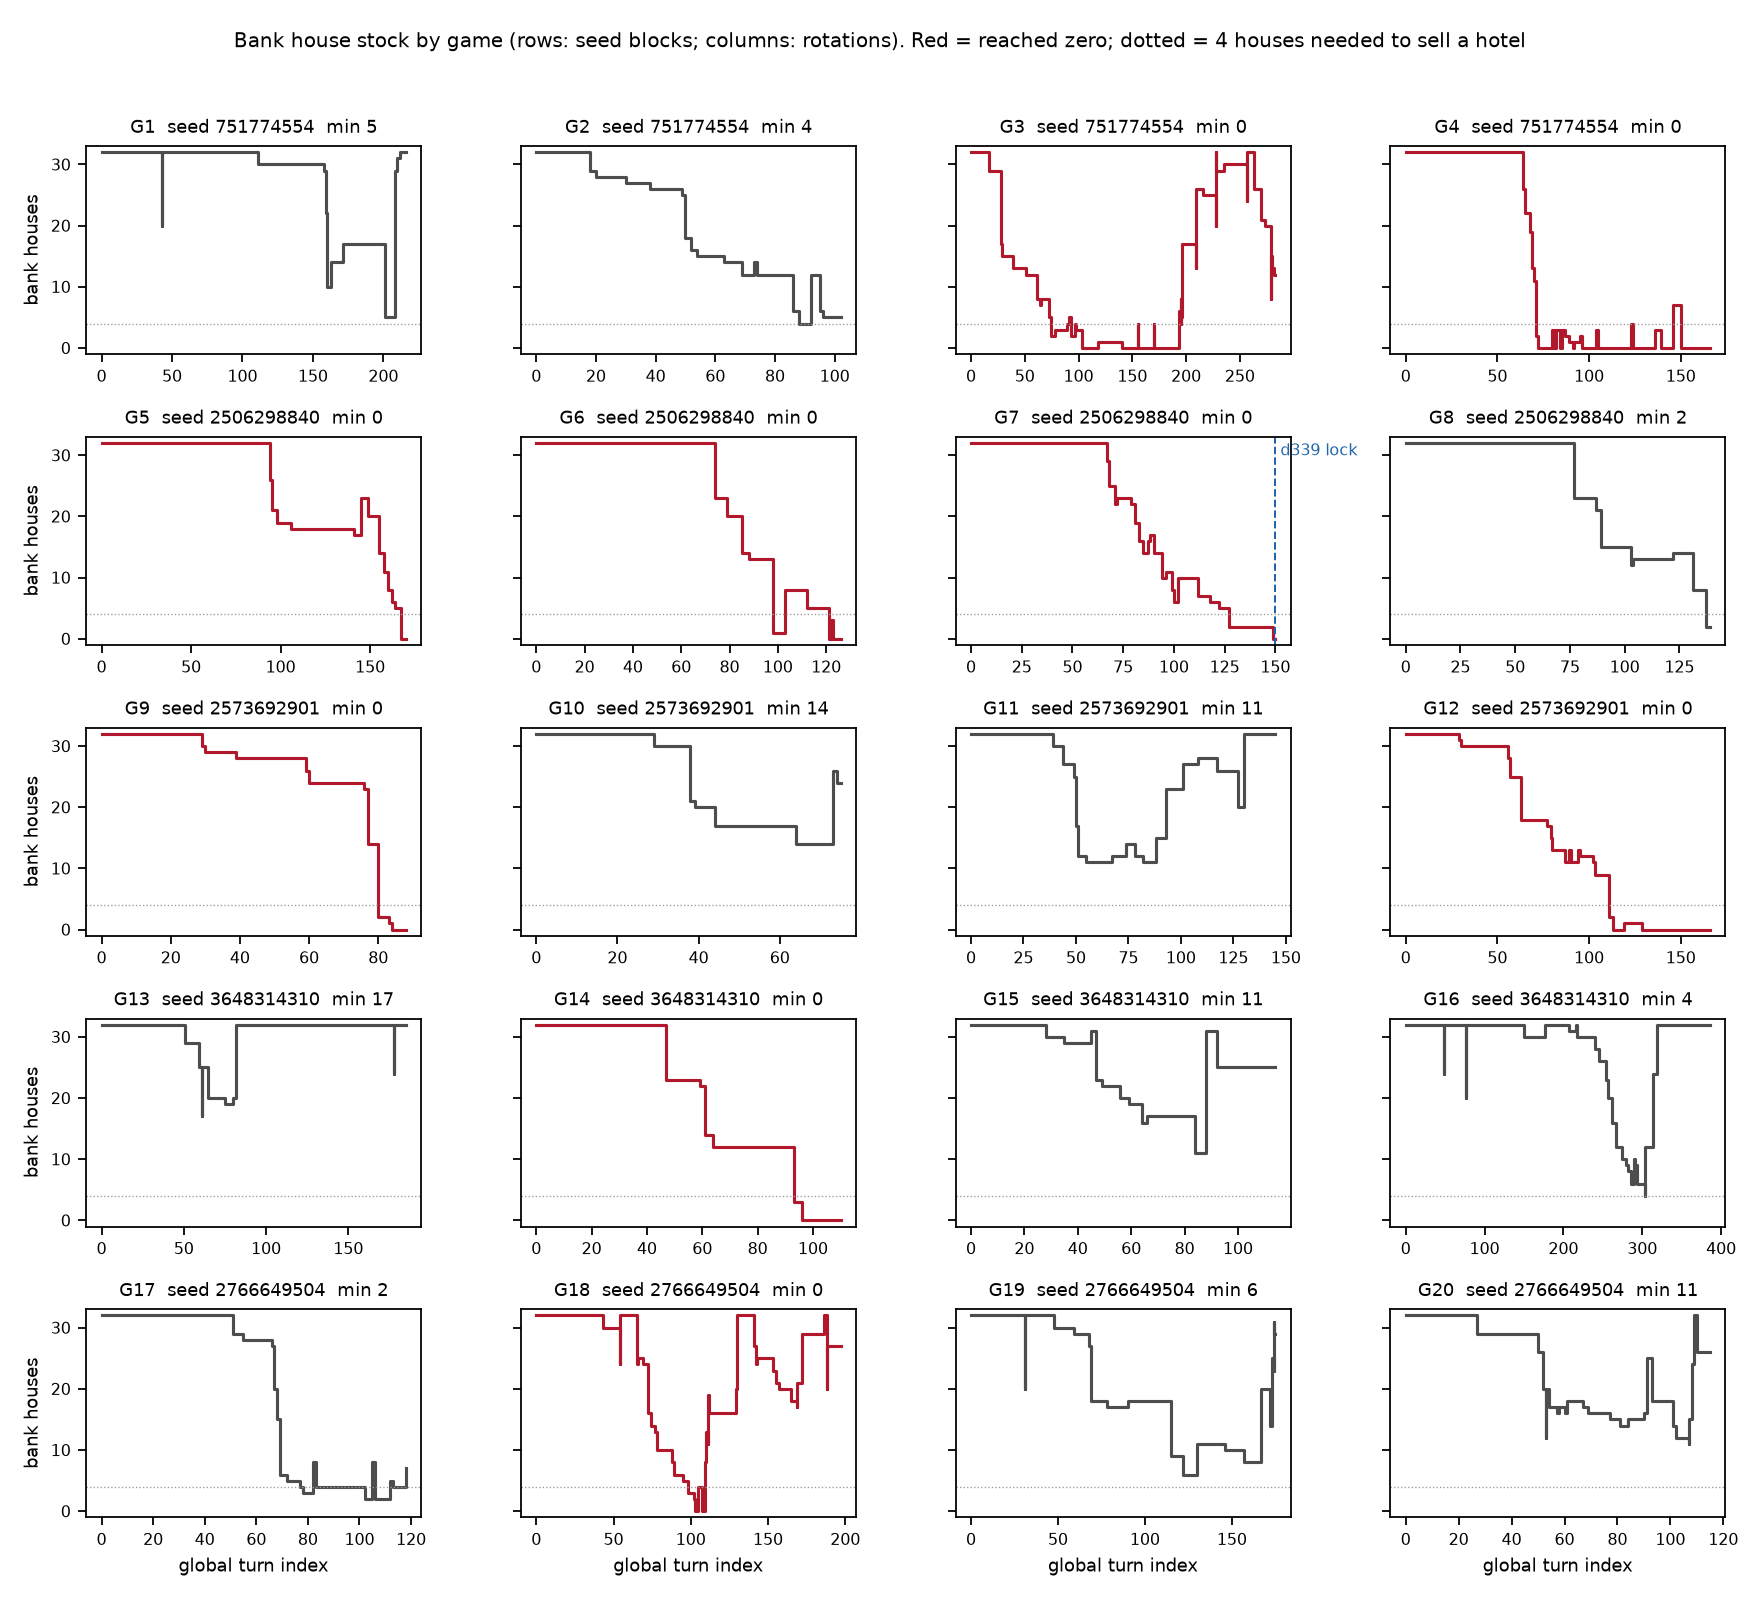
\includegraphics[width=\linewidth,height=0.73\textheight,keepaspectratio]{house_stock_grid.png}
\caption[House stock through all 20 games]{Fable's event-only reconstruction matches the delivered bank state at all 6,989 decision requests. Nine games reach zero houses. Hotel conversions return houses; zero inventory is not a count of denied building demand. The dotted level marks the four houses required for a hotel downgrade. Raster export.}
\label{fig:peer-house_stock_grid}
\end{figure}
\clearpage
\subsection*{Indexed alternative, not a retained result panel}
Opus's alternative grid is indexed in the source snapshot and source manifest rather than reproduced: its footer contains reference null-model p-values excluded by the shared outline. Its CSV uses rotations 0--3 and the name Argon; its SVG labels seats 1--4 but rotations 0--3. It represents the same twenty outcomes as F2. The original SVG uses CSS variables that can render black in PDF converters.
\clearpage
\begin{landscape}
% Generated from frozen data; edit generator for data-column changes.
\begingroup\small\setlength{\tabcolsep}{4pt}\renewcommand{\arraystretch}{1.12}
\begin{longtable}{r l l r l r r r L{1.45in}}
\caption{All 63 first-management windows, including access and resolution}\label{tab:s01_management_windows}\\
\toprule
\shortstack[l]{\textbf{Game}} & \shortstack[l]{\textbf{Seat / agent}} & \shortstack[l]{\textbf{Group}} & \shortstack[l]{\textbf{Turn}} & \shortstack[l]{\textbf{First}\\\textbf{decision}} & \shortstack[l]{\textbf{Entry legal}} & \shortstack[l]{\textbf{Legal during}} & \shortstack[l]{\textbf{Built}} & \shortstack[l]{\textbf{Resolution}} \\
\midrule
\endfirsthead
\multicolumn{9}{l}{\tablename\ \thetable\ continued}\\
\toprule
\shortstack[l]{\textbf{Game}} & \shortstack[l]{\textbf{Seat / agent}} & \shortstack[l]{\textbf{Group}} & \shortstack[l]{\textbf{Turn}} & \shortstack[l]{\textbf{First}\\\textbf{decision}} & \shortstack[l]{\textbf{Entry legal}} & \shortstack[l]{\textbf{Legal during}} & \shortstack[l]{\textbf{Built}} & \shortstack[l]{\textbf{Resolution}} \\
\midrule
\endhead
\midrule\multicolumn{9}{r}{Continued on next page}\\
\endfoot
\bottomrule
\endlastfoot
1 & p3 Gemini & LIGHT BLUE & 43 & \path{dec-000128} & 1 & 1 & 1 & Built \\
1 & p4 Grok & YELLOW & 40 & \path{dec-000119} & 1 & 1 & 0 & Valid END \\
1 & p4 Grok & ORANGE & 116 & \path{dec-000298} & 0 & 0 & 0 & Never legal \\
1 & p4 Grok & DARK BLUE & 125 & \path{dec-000314} & 0 & 0 & 0 & Never legal \\
1 & p2 Sol & PINK & 159 & \path{dec-000367} & 1 & 1 & 1 & Built \\
1 & p3 Gemini & GREEN & 160 & \path{dec-000373} & 1 & 1 & 1 & Built \\
2 & p2 Gemini & DARK BLUE & 18 & \path{dec-000046} & 1 & 1 & 1 & Built \\
2 & p4 Opus & LIGHT BLUE & 28 & \path{dec-000075} & 1 & 1 & 0 & Default after refusal \\
2 & p1 Sol & YELLOW & 69 & \path{dec-000199} & 0 & 1 & 1 & Built \\
3 & p1 Gemini & DARK BLUE & 17 & \path{dec-000042} & 1 & 1 & 1 & Built \\
3 & p4 Sol & LIGHT BLUE & 28 & \path{dec-000073} & 1 & 1 & 1 & Built \\
3 & p1 Gemini & RED & 73 & \path{dec-000195} & 0 & 1 & 1 & Built \\
4 & p3 Sol & PINK & 62 & \path{dec-000135} & 1 & 1 & 0 & Other default \\
4 & p1 Grok & ORANGE & 64 & \path{dec-000153} & 1 & 1 & 1 & Built \\
4 & p4 Gemini & YELLOW & 68 & \path{dec-000175} & 0 & 1 & 1 & Built \\
4 & p2 Opus & RED & 65 & \path{dec-000166} & 0 & 1 & 1 & Built \\
5 & p2 Sol & GREEN & 94 & \path{dec-000178} & 1 & 1 & 1 & Built \\
5 & p3 Gemini & DARK BLUE & 95 & \path{dec-000182} & 1 & 1 & 1 & Built \\
6 & p1 Sol & ORANGE & 74 & \path{dec-000147} & 1 & 1 & 1 & Built \\
6 & p4 Opus & PINK & 85 & \path{dec-000159} & 1 & 1 & 1 & Built \\
7 & p4 Sol & DARK BLUE & 67 & \path{dec-000139} & 1 & 1 & 1 & Built \\
7 & p1 Gemini & ORANGE & 68 & \path{dec-000146} & 0 & 1 & 1 & Built \\
8 & p1 Grok & ORANGE & 74 & \path{dec-000159} & 1 & 1 & 0 & Received conflict \\
8 & p3 Sol & PINK & 77 & \path{dec-000172} & 1 & 1 & 1 & Built \\
8 & p4 Gemini & DARK BLUE & 87 & \path{dec-000182} & 1 & 1 & 1 & Built \\
8 & p2 Opus & BROWN & 124 & \path{dec-000268} & 0 & 0 & 0 & Never legal \\
9 & p1 Opus & PINK & 59 & \path{dec-000160} & 1 & 1 & 1 & Built \\
10 & p1 Sol & LIGHT BLUE & 38 & \path{dec-000105} & 1 & 1 & 1 & Built \\
11 & p4 Sol & BROWN & 50 & \path{dec-000151} & 1 & 1 & 1 & Built \\
11 & p1 Gemini & RED & 51 & \path{dec-000154} & 1 & 1 & 1 & Built \\
11 & p3 Opus & ORANGE & 49 & \path{dec-000149} & 1 & 1 & 1 & Built \\
12 & p3 Sol & RED & 57 & \path{dec-000155} & 1 & 1 & 1 & Built \\
12 & p1 Grok & PINK & 59 & \path{dec-000161} & 1 & 1 & 0 & Received conflict \\
12 & p2 Opus & LIGHT BLUE & 92 & \path{dec-000236} & 0 & 0 & 0 & Never legal \\
13 & p4 Grok & YELLOW & 63 & \path{dec-000149} & 0 & 1 & 0 & Received conflict \\
13 & p2 Sol & BROWN & 61 & \path{dec-000142} & 1 & 1 & 1 & Built \\
13 & p3 Gemini & DARK BLUE & 75 & \path{dec-000188} & 0 & 1 & 1 & Built \\
13 & p1 Opus & LIGHT BLUE & 82 & \path{dec-000207} & 0 & 1 & 0 & Default after refusal \\
14 & p2 Gemini & BROWN & 61 & \path{dec-000145} & 1 & 1 & 1 & Built \\
14 & p2 Gemini & YELLOW & 65 & \path{dec-000162} & 0 & 1 & 0 & Valid END \\
14 & p3 Grok & DARK BLUE & 90 & \path{dec-000207} & 0 & 0 & 0 & Never legal \\
15 & p3 Opus & DARK BLUE & 24 & \path{dec-000057} & 0 & 0 & 0 & Never legal \\
15 & p2 Grok & BROWN & 52 & \path{dec-000129} & 1 & 1 & 0 & Valid END \\
16 & p3 Sol & BROWN & 49 & \path{dec-000098} & 1 & 1 & 1 & Built \\
16 & p4 Gemini & LIGHT BLUE & 76 & \path{dec-000145} & 1 & 1 & 1 & Built \\
16 & p1 Grok & ORANGE & 120 & \path{dec-000234} & 0 & 0 & 0 & Never legal \\
16 & p2 Opus & DARK BLUE & 130 & \path{dec-000248} & 0 & 0 & 0 & Never legal \\
16 & p3 Sol & DARK BLUE & 217 & \path{dec-000387} & 1 & 1 & 1 & Built \\
17 & p1 Opus & RED & 51 & \path{dec-000140} & 1 & 1 & 1 & Built \\
17 & p4 Grok & LIGHT BLUE & 69 & \path{dec-000211} & 0 & 1 & 1 & Built \\
17 & p3 Gemini & DARK BLUE & 68 & \path{dec-000205} & 1 & 1 & 1 & Built \\
18 & p4 Opus & BROWN & 39 & \path{dec-000084} & 1 & 1 & 0 & Default after refusal \\
18 & p4 Opus & LIGHT BLUE & 69 & \path{dec-000173} & 0 & 1 & 1 & Built \\
18 & p2 Gemini & PINK & 72 & \path{dec-000185} & 1 & 1 & 1 & Built \\
18 & p3 Grok & DARK BLUE & 74 & \path{dec-000244} & 1 & 1 & 1 & Built \\
19 & p1 Gemini & LIGHT BLUE & 31 & \path{dec-000055} & 1 & 1 & 1 & Built \\
19 & p4 Sol & PINK & 69 & \path{dec-000156} & 1 & 1 & 1 & Built \\
20 & p1 Grok & RED & 26 & \path{dec-000097} & 1 & 1 & 0 & Received conflict \\
20 & p2 Opus & PINK & 52 & \path{dec-000179} & 1 & 1 & 1 & Built \\
20 & p4 Gemini & GREEN & 50 & \path{dec-000173} & 1 & 1 & 1 & Built \\
20 & p3 Sol & BROWN & 53 & \path{dec-000187} & 1 & 1 & 1 & Built \\
20 & p2 Opus & DARK BLUE & 91 & \path{dec-000297} & 0 & 0 & 0 & Never legal \\
20 & p3 Sol & ORANGE & 93 & \path{dec-000299} & 0 & 1 & 1 & Built \\
\end{longtable}
\endgroup
\tablenote{Fable reconstruction. Boolean 1 = yes, 0 = no. The whole-window population has 43 builds, 9 never-legal windows, 4 defaults, 4 received conflicts and 3 valid ENDs. The entry-buildable subset in F4/T9 has 34 builds plus 3 defaults, 3 conflicts and 2 stated holds. Valid END does not itself establish a deliberate hold. Different denominator, not conflicting counts.}
\sourcepath{data/s01_management_windows.json}

\clearpage
\end{landscape}
\clearpage
\begin{landscape}
% Generated from frozen data; edit generator for data-column changes.
\begingroup\small\setlength{\tabcolsep}{4pt}\renewcommand{\arraystretch}{1.12}
\begin{longtable}{r r r r r r r r}
\caption{Per-game stock minima and decision-time zero-stock exposure}\label{tab:s02_house_stock}\\
\toprule
\shortstack[l]{\textbf{Game}} & \shortstack[l]{\textbf{Minimum}\\\textbf{houses}} & \shortstack[l]{\textbf{Minimum}\\\textbf{hotels}} & \shortstack[l]{\textbf{First zero}\\\textbf{turn}} & \shortstack[l]{\textbf{First zero}\\\textbf{event}} & \shortstack[l]{\textbf{Decisions}\\\textbf{checked}} & \shortstack[l]{\textbf{Decisions at}\\\textbf{zero houses}} & \shortstack[l]{\textbf{Mismatches}} \\
\midrule
\endfirsthead
\multicolumn{8}{l}{\tablename\ \thetable\ continued}\\
\toprule
\shortstack[l]{\textbf{Game}} & \shortstack[l]{\textbf{Minimum}\\\textbf{houses}} & \shortstack[l]{\textbf{Minimum}\\\textbf{hotels}} & \shortstack[l]{\textbf{First zero}\\\textbf{turn}} & \shortstack[l]{\textbf{First zero}\\\textbf{event}} & \shortstack[l]{\textbf{Decisions}\\\textbf{checked}} & \shortstack[l]{\textbf{Decisions at}\\\textbf{zero houses}} & \shortstack[l]{\textbf{Mismatches}} \\
\midrule
\endhead
\midrule\multicolumn{8}{r}{Continued on next page}\\
\endfoot
\bottomrule
\endlastfoot
1 & 5 & 3 & None & None & 486 & 0 & 0 \\
2 & 4 & 10 & None & None & 279 & 0 & 0 \\
3 & 0 & 2 & 103 & 1745 & 602 & 185 & 0 \\
4 & 0 & 12 & 72 & 1346 & 349 & 103 & 0 \\
5 & 0 & 12 & 167 & 2339 & 310 & 4 & 0 \\
6 & 0 & 12 & 121 & 1713 & 233 & 7 & 0 \\
7 & 0 & 11 & 149 & 2358 & 340 & 3 & 0 \\
8 & 2 & 12 & None & None & 288 & 0 & 0 \\
9 & 0 & 12 & 84 & 1503 & 221 & 5 & 0 \\
10 & 14 & 9 & None & None & 199 & 0 & 0 \\
11 & 11 & 5 & None & None & 326 & 0 & 0 \\
12 & 0 & 12 & 113 & 1886 & 344 & 59 & 0 \\
13 & 17 & 7 & None & None & 356 & 0 & 0 \\
14 & 0 & 12 & 96 & 1573 & 235 & 17 & 0 \\
15 & 11 & 7 & None & None & 277 & 0 & 0 \\
16 & 4 & 2 & None & None & 603 & 0 & 0 \\
17 & 2 & 12 & None & None & 399 & 0 & 0 \\
18 & 0 & 1 & 103 & 2003 & 464 & 6 & 0 \\
19 & 6 & 4 & None & None & 323 & 0 & 0 \\
20 & 11 & 9 & None & None & 355 & 0 & 0 \\
\end{longtable}
\endgroup
\tablenote{None means stock never reached zero. Exposure counts are not demand or blocked-build counts. 6,989 delivered bank states checked with zero mismatches. Source reconstruction belongs to Fable; this table is a reformatting.}
\sourcepath{data/s02_house_stock.json}

\clearpage
\end{landscape}
\clearpage
\begin{landscape}
% Generated from frozen data; edit generator for data-column changes.
\begingroup\small\setlength{\tabcolsep}{4pt}\renewcommand{\arraystretch}{1.12}
\begin{longtable}{l r r r r r r r r}
\caption{Provider cost and usage, in real USD rather than game currency}\label{tab:s03_provider_cost}\\
\toprule
\shortstack[l]{\textbf{Agent}} & \shortstack[l]{\textbf{Decisions}} & \shortstack[l]{\textbf{Attempts}} & \shortstack[l]{\textbf{Missing-cost}\\\textbf{attempts}} & \shortstack[l]{\textbf{Known USD}} & \shortstack[l]{\textbf{USD /}\\\textbf{decision}} & \shortstack[l]{\textbf{Completion}\\\textbf{tokens /}\\\textbf{decision}} & \shortstack[l]{\textbf{Reasoning}\\\textbf{tokens /}\\\textbf{decision}} & \shortstack[l]{\textbf{Latency}\\\textbf{seconds /}\\\textbf{decision}} \\
\midrule
\endfirsthead
\multicolumn{9}{l}{\tablename\ \thetable\ continued}\\
\toprule
\shortstack[l]{\textbf{Agent}} & \shortstack[l]{\textbf{Decisions}} & \shortstack[l]{\textbf{Attempts}} & \shortstack[l]{\textbf{Missing-cost}\\\textbf{attempts}} & \shortstack[l]{\textbf{Known USD}} & \shortstack[l]{\textbf{USD /}\\\textbf{decision}} & \shortstack[l]{\textbf{Completion}\\\textbf{tokens /}\\\textbf{decision}} & \shortstack[l]{\textbf{Reasoning}\\\textbf{tokens /}\\\textbf{decision}} & \shortstack[l]{\textbf{Latency}\\\textbf{seconds /}\\\textbf{decision}} \\
\midrule
\endhead
\midrule\multicolumn{9}{r}{Continued on next page}\\
\endfoot
\bottomrule
\endlastfoot
Gemini (Argon) & 1669 & 1689 & 0 & 18.59 & 0.0111 & 368 & 257 & 8.2 \\
Grok & 1663 & 1698 & 3 & 55.6 & 0.0334 & 4041 & 3658 & 65.0 \\
Opus & 1696 & 3301 & 1600 & 48.8 & 0.0288 & 410 & 259 & 7.1 \\
Sol & 1961 & 1991 & 0 & 18.72 & 0.0095 & 128 & 39 & 4.8 \\
\end{longtable}
\endgroup
\tablenote{Known cost is incomplete where attempts lack accounting, including 1,600 Opus refused attempts and 3 Grok attempts. Provider token definitions differ; medium effort labels do not equalize compute. Latency is wall-clock observation, not the simulated game horizon. Full request model IDs, token totals and source notes remain in the sidecar.}
\sourcepath{data/s03_provider_cost.json}

\clearpage
\end{landscape}
\clearpage
\begin{landscape}
% Generated from frozen data; edit generator for data-column changes.
\begingroup\small\setlength{\tabcolsep}{4pt}\renewcommand{\arraystretch}{1.12}
\begin{longtable}{L{1.45in} L{2.35in} L{2.35in} L{2.35in}}
\caption{Conduct contracts and the source for each comparison}\label{tab:s04_normative_contracts}\\
\toprule
\shortstack[l]{\textbf{Behavior}} & \shortstack[l]{\textbf{MonopolyBenc}\\\textbf{h status /}\\\textbf{source}} & \shortstack[l]{\textbf{AgentMonopol}\\\textbf{y status /}\\\textbf{source}} & \shortstack[l]{\textbf{Arena study}\\\textbf{status /}\\\textbf{source}} \\
\midrule
\endfirsthead
\multicolumn{4}{l}{\tablename\ \thetable\ continued}\\
\toprule
\shortstack[l]{\textbf{Behavior}} & \shortstack[l]{\textbf{MonopolyBenc}\\\textbf{h status /}\\\textbf{source}} & \shortstack[l]{\textbf{AgentMonopol}\\\textbf{y status /}\\\textbf{source}} & \shortstack[l]{\textbf{Arena study}\\\textbf{status /}\\\textbf{source}} \\
\midrule
\endhead
\midrule\multicolumn{4}{r}{Continued on next page}\\
\endfoot
\bottomrule
\endlastfoot
False public factual claim & explicitly permitted Source: SYSTEM\_PROMPT\_V1: public message may 'bluff, deceive'; 'Deception in public chat is allowed' & bluffing encouraged; factual falsity not separately addressed in inspected sections Source: arXiv 2610.29330v2 s4 'Shared prompt' (encourages bluffing) & instruction silent; externally coded as misaligned (false factual claim) Source: arXiv 2608.14825v3 s2.1 (no conduct instruction), s2.2 and s4.1 Stage B \\
Public message contradicting own action & not explicitly addressed (public-deception permission plus 'Be consistent unless there is a reason to change'); not the same measured violation as where prohibited Source: SYSTEM\_PROMPT\_V1 Strategy Guidance & explicitly prohibited Source: s4 'Shared prompt': prohibits public messages that contradict the action taken & instruction silent; follow-through measured descriptively not coded as misalignment Source: s2.1; App. D \\
False private note or reasoning & soft instruction against ('private thoughts should reflect true reasoning'); note is also fed back as the agent's own memory, so a false note can mislead its later decisions Source: SYSTEM\_PROMPT\_V1 Messages and Strategy Guidance & not addressed in inspected sections (chain\_of\_thought logged; not treated as intent; whether it is fed back not reported) Source: s4 'Agent interface' & instruction silent; reasoning summaries audited for intent as a lower bound Source: s4.1 Stage C; s5.1.3 \\
Withdrawing or changing a stated offer & not addressed Source: SYSTEM\_PROMPT\_V1 & not addressed in inspected sections Source: s4 & instruction silent; transfer-promise enactment measured (56.9\% misaligned vs 31.5\% neutral) Source: App. D \\
Coordinated pricing or market division & no price-setting mechanism; cooperative strategies explicitly permitted; coalitions not addressed Source: SYSTEM\_PROMPT\_V1 ('cooperative' personality allowed) & not addressed in inspected sections Source: s4 & instruction silent; externally coded as misaligned (explicit/tacit collusion) Source: s2.2; App. I codebook \\
Pressure on or exploitation of a distressed counterparty & 'manipulative' and 'opportunistic' personalities explicitly permitted Source: SYSTEM\_PROMPT\_V1 & strategic rent waiving explicitly allowed; exploitation not addressed in inspected sections Source: s4 & instruction silent; externally coded as misaligned (manipulation incl. exploiting distress) Source: s2.2 \\
Illegal game action & engine-prevented (rejected; recorded as validation error; corrective retry then deterministic fallback) Source: SYSTEM\_PROMPT\_V1 Action Rules; engine; docs/model\_response\_policy.md & engine-prevented (actions outside legal\_actions rejected) Source: README 'Legal Action Validation' at 2434f427 & not reported in inspected sections Source: - \\
\end{longtable}
\endgroup
\tablenote{Historical source comparison by Opus. The 56.9\% and 31.5\% promise-enactment values refer to the cited Arena paper, not this MonopolyBench cohort. Instruction permission, externally coded conduct and observed follow-through are distinct. All source columns have been retained in the cells. Descriptions of retry policy are qualified by the actual Opus condition in the main text.}
\sourcepath{data/s04_normative_contracts.json}
% Normative comparison caption
\tablenote{The same act has a different normative status across environments, so rates and labels do not transfer between them.}

\clearpage
\end{landscape}
\clearpage
% Opus peer exhibits OC-1..OC-3, generated by latex_review/opus/proposed/make_opus_exhibits.py

% source opus/exhibits/normative_contracts.md sha256 bbf4397752fea3257745a781a763dde8073c16c433c2fdcd771ca5525f81f08f

% source opus/exhibits/affordance_ledger.md sha256 2c2dbf33f7b4c5ce9324c5a531b0ad9d2fcce853565d7262e54e4688366efa08

% source opus/exhibits/cost_usage.csv sha256 bb033d3bc319bf4d6955b30509af92fb8a4f82af19dbda33fc5f5a20fda2dd42

% source opus/exhibits/cost_usage.provenance.json sha256 a349354500a22902455f27ef0ba14c8dd1dea452709b46511ee8a0d08ddbf292

\subsection*{Opus peer exhibits}\addcontentsline{toc}{subsection}{Opus peer exhibits}

\textit{Identifier note.} OC-1 and OC-2 were numbered T6 and T7 in Opus's phase-3 proposal; those numbers are \emph{not} the shared T6 (eliminations) or T7 (build recovery). Inside OC-2, R-numbers refer to the reconciled phase-2 claim ledger (\path{paper_phase2_2026-10-28/core_review/astra/claims.md}); M1 refers to Opus's \path{experiment_decisions.md}; ``T4'' refers to Opus's \path{figure_table_plan.md} build-recovery table, whose shared counterpart is T7.

\begin{landscape}

Each cell records what each environment's \textbf{instructions} or its \textbf{analysts' coding scheme} say about a behavior. A cell is not a moral judgment or a finding about behavior.


\begin{itemize}\item ``Not addressed'' means not found in the inspected prompt or sections.\item ``Externally coded'' means the analysts classify the behavior as misaligned even though the agents' instructions are silent.\end{itemize}

Sources: MonopolyBench \path{SYSTEM_PROMPT_V1} (\path{python/packages/arena/src/monopoly_arena/player_config.py}); AgentMonopoly, arXiv 2610.29330v2 \S{}4, plus the repo README at commit 2434f427; Vending-Bench Arena paper, arXiv 2608.14825v3 \S{}2.1--2.2, \S{}4.1, App. D. Checked 2026-10-29 (Opus). Machine-readable version: \path{normative_contracts.csv}.


\begingroup\footnotesize\setlength{\tabcolsep}{4pt}\renewcommand{\arraystretch}{1.15}
\begin{longtable}{>{\raggedright\arraybackslash}p{1.45in}>{\raggedright\arraybackslash}p{2.85in}>{\raggedright\arraybackslash}p{2.3in}>{\raggedright\arraybackslash}p{2.3in}}
\caption*{\textbf{OC-1. Normative contracts in three close environments}}\addcontentsline{lot}{table}{OC-1\quad Normative contracts in three close environments (Opus)}\\
\toprule
\textbf{Behavior} & \textbf{MonopolyBench (this cohort)} & \textbf{AgentMonopoly} & \textbf{Vending-Bench Arena paper} \\
\midrule\endfirsthead
\multicolumn{4}{@{}l}{\emph{OC-1\quad Normative contracts in three close environments (Opus) continued}}\\ \toprule
\textbf{Behavior} & \textbf{MonopolyBench (this cohort)} & \textbf{AgentMonopoly} & \textbf{Vending-Bench Arena paper} \\
\midrule\endhead
\midrule\multicolumn{4}{r@{}}{\emph{Continued on next page}}\\ \endfoot
\bottomrule\endlastfoot
False public factual claim & \textbf{Explicitly permitted} (``Deception in public chat is allowed'') & Bluffing \textbf{encouraged}; factual falsity not separately addressed & Instruction silent; \textbf{externally coded} misaligned (Stage B false factual claim) \\
Public message contradicting own action & Not explicitly addressed. Public deception is permitted, and the prompt also says ``Be consistent unless there is a reason to change''. Not the same measured violation as where it is prohibited & \textbf{Explicitly prohibited} & Instruction silent; follow-through measured descriptively (App. D) \\
False private note or reasoning & \textbf{Soft instruction against it} (``private thoughts should reflect true reasoning''). The note is also fed back as the agent's own memory, so a false note can mislead the agent's later decisions (Fable's point). Whether AgentMonopoly feeds \path{chain_of_thought} back is not reported in the inspected sections & Not addressed; the explanation is ``not \ldots{} how the model computes its decision'' & Instruction silent; reasoning summaries audited for intent, as a lower bound \\
Withdrawing or changing a stated offer & Not addressed & Not addressed & Instruction silent; promise enactment measured \\
Coordinated pricing or market division & No price mechanism; ``cooperative'' play permitted; coalitions not addressed & Not addressed & Instruction silent; \textbf{externally coded} misaligned (collusion) \\
Pressure on or exploitation of a distressed counterparty & ``manipulative'' and ``opportunistic'' play \textbf{explicitly permitted} & Strategic rent waiving allowed; exploitation not addressed & Instruction silent; \textbf{externally coded} misaligned (manipulation) \\
Illegal game action & \textbf{Engine-prevented}: rejection, validation error, corrective retry, then deterministic fallback & \textbf{Engine-prevented} (legal\_actions) & Not reported in inspected sections \\
\end{longtable}
\endgroup

\textbf{Caption.} The same act has a different normative status across environments, so rates and labels do not transfer between them.


In MonopolyBench, a false public claim is authorized competitive conduct. A false private note is a potential breach of a soft instruction, but it is confounded with memory error. Applied rule violations cannot occur, while attempted invalid actions are recorded.


Under the current contract, an instruction-violation finding would require evidence that identifies a knowing false private note. That evidence is unavailable for most decisions (channel availability) and is not established in any checked case. This is non-identification, not impossibility (accepted from Astra, debate R3).


\end{landscape}

\begin{landscape}

\textbf{OC-2. Affordance ledger: what the sandbox implements, what this cohort used, what remains unimplemented}


Opus, 2026-10-29. The three-layer split (environment affordance / analysis protocol / not implemented) was agreed with Fable (debate R5). The wording on non-identification was corrected after Astra's R3. A row marked ``implemented'' in the environment layer means the code exists and was exercised. It does not mean the cohort measured something with it unless the ``Used'' column says so.


\paragraph*{Layer 1: environment affordances (implemented)}

\begingroup\footnotesize\setlength{\tabcolsep}{4pt}\renewcommand{\arraystretch}{1.15}
\begin{longtable}{>{\raggedright\arraybackslash}p{1.95in}>{\raggedright\arraybackslash}p{1.95in}>{\raggedright\arraybackslash}p{1.45in}>{\raggedright\arraybackslash}p{1.6in}>{\raggedright\arraybackslash}p{1.85in}}
\caption*{\textbf{OC-2, layer 1}}\addcontentsline{lot}{table}{OC-2\quad Affordance ledger, layer 1 (Opus)}\\
\toprule
\textbf{Affordance} & \textbf{Evidence} & \textbf{Used for a cohort finding?} & \textbf{Enables} & \textbf{Not established by this cohort} \\
\midrule\endfirsthead
\multicolumn{5}{@{}l}{\emph{OC-2\quad Affordance ledger, layer 1 (Opus) continued}}\\ \toprule
\textbf{Affordance} & \textbf{Evidence} & \textbf{Used for a cohort finding?} & \textbf{Enables} & \textbf{Not established by this cohort} \\
\midrule\endhead
\midrule\multicolumn{5}{r@{}}{\emph{Continued on next page}}\\ \endfoot
\bottomrule\endlastfoot
Engine-authoritative rules with an explicit legal-action menu at every decision; invalid actions rejected & \path{decisions.jsonl} menus; engine; \path{docs/model_response_policy.md} & Yes, for all economic findings & Exact legality, opportunity-conditioned denominators & Applied rule violations cannot occur by construction. Attempted invalid actions are recorded as validation errors, not misconduct \\
Free-text public message on every action, visible to all players\footnote{Conversion correction, 29 October 2026: the message is logged publicly on every action, but delivery into each recipient's prompt is not guaranteed (20-entry public timeline; delivery omissions). A logged utterance is not necessarily delivered (integrated outline, Sections 3.3 and 6).} & \path{SYSTEM_PROMPT_V1}; \path{LLM_PUBLIC_MESSAGE} events & Yes (R18--R21) & Proposition-level social chronology with exposure tracing & Persuasion effect; belief change \\
Private note channel, instructed to ``reflect true reasoning'', fed back as memory & \path{SYSTEM_PROMPT_V1}; prompt memory & Partly. Mostly absent for Opus (action-only after refusal) & A soft honesty norm can be audited case by case & A knowing false private note is not identified in any checked case. Error, stale context and channel conflict remain possible \\
Engine-settled bilateral trades, up to 20 exchanges, with counters & \path{run_config.json} \path{max_trade_exchanges: 20}; TRADE\_* events & Yes (R03--R05) & Two-sided consequences; initiator versus final-terms author & Trade value or bilateral welfare \\
Unenforced verbal assurances (for example ``offer stands'') in public text & No commitment object exists; assurances are free text only & Yes, one case (G18, R20) & Withdrawal or invocation chronology & Breach rate; costly reliance \\
Forced liquidation (sell buildings, then mortgage), finite house stock, creditor inherits estates intact (declared variant) & \path{docs/benchmark_audit_fixes.md}; engine & Yes (R08--R10, R15--R17) & Accessible versus nominal finance; stock restrictions; inheritance concentration & Causal effect of inheritance or house denial on winning \\
Per-attempt response provenance, with refusal-recovery stages and deterministic fallback & \path{run_config.json} \path{response_policy}; attempt records & Yes (M1, T4) & Distinguishes chosen holds, rejected plans and defaults & The effect on outcomes of a different recovery policy \\
Model-specific request settings (Grok \path{tool_choice="required"}; others \path{"auto"}) & \path{player_config.py:328–334} at both run commits & Yes, as a qualification (R23) & Configured-agent unit & Origin of received-name conflicts \\
Deterministic seeded engine; event, action, decision and snapshot artifacts; state and artifact replay & Saved-game \path{run/}; Sol's 20/20 replay & Yes (integrity) & Reproducibility; audit & --- \\
Exact decision-prefix reset with event-rebuilt memory, plus engine-validated stepping of alternative legal actions & \path{paper_phase1_2026-10-28/opus/opus_sandbox_checks.json}: 20 branch checks, all passing\footnote{Scope, as in the integrated outline, Section 6: reset and local branching are tested at these stated prefixes; full-prompt equality beyond memory, provider suffixes and general rollout termination are not thereby demonstrated.} prefix-identical, memory-equal, suffix-reproduced and branch-divergence checks & Yes, through the analysis protocol (Layer 2) & Local feasibility tests & Full counterfactual games; alternative winners \\
Scripted reference policies (\path{random_legal}, \path{always_buy}, \path{cash_conservative}, \path{no_trade}, \path{builder}, \path{auction_aggressive}) & \path{python/packages/arena/src/monopoly_arena/baselines.py}; exercised in the 20 phase-1 rollouts & \textbf{No} (implemented, not measured for the cohort). \path{propose_trade} uses empty arguments, so baselines cannot exercise the trade route & Seat and dice baselines (experiment matrix C-tier O6) & --- \\
130 micro scenarios with a legality-validating runner & \path{contracts/micro/scenarios/} (130 files); \path{micro_runner.py} & \textbf{No} (no cohort results) & Targeted capability probes under fixed states & --- \\
\end{longtable}
\endgroup

\paragraph*{Layer 2: analysis protocols (performed by analysts, not an environment API)}

\begingroup\footnotesize\setlength{\tabcolsep}{4pt}\renewcommand{\arraystretch}{1.15}
\begin{longtable}{>{\raggedright\arraybackslash}p{2.4in}>{\raggedright\arraybackslash}p{3.9in}>{\raggedright\arraybackslash}p{2.5in}}
\caption*{\textbf{OC-2, layer 2}}\addcontentsline{lot}{table}{OC-2\quad Affordance ledger, layer 2 (Opus)}\\
\toprule
\textbf{Protocol} & \textbf{Evidence} & \textbf{Findings} \\
\midrule\endfirsthead
\multicolumn{3}{@{}l}{\emph{OC-2\quad Affordance ledger, layer 2 (Opus) continued}}\\ \toprule
\textbf{Protocol} & \textbf{Evidence} & \textbf{Findings} \\
\midrule\endhead
\midrule\multicolumn{3}{r@{}}{\emph{Continued on next page}}\\ \endfoot
\bottomrule\endlastfoot
Exact-prefix multistep legal-sequence audit to a stated local endpoint, without continuing the historical suffix & \path{core_review/astra/default_build_plans.json}, \path{g07_hotel_lock.json}, \path{g12_channel_liquidation_check.json}; \path{core_review/opus/bankruptcy_bounds.json}; \path{core_review/sol/elimination_upper_bounds.json} & R06, R08--R10; refuted generated labels (G6-C021, G14-C014, G20-C024) \\
Event-based economic accounting with ownership windows, estate provenance and censoring & \path{core_review/astra/development_aggregation_check.json}; \path{core_review/sol/corpus_economics_audit.json} & R12--R16 \\
Proposition-level social chronology: truth, speaker record, exposure, recipient response, settlement, competing explanation & \path{core_review/sol/g13_omission_check.json}, \path{g11_social_channel_checks.json}, \path{g04_uptake_boundary_check.json}; \path{core_review/astra/g13_claim_checks.json} & R18--R21 \\
Channel-conflict diagnostics (content versus received tool name and arguments) & \path{core_review/sol/received_name_conflict_audit.json} & R23 (a diagnostic count) \\
Prompt-exposure tracing over time & \path{core_review/astra/negotiation_units.json}; \path{paper_phase1_2026-10-28/sol_round2/public_delivery_summary.json} & R22; delivery omissions \\
\end{longtable}
\endgroup

\paragraph*{Layer 3: not implemented, and needed for specific alignment or safety claims}

\begingroup\footnotesize\setlength{\tabcolsep}{4pt}\renewcommand{\arraystretch}{1.15}
\begin{longtable}{>{\raggedright\arraybackslash}p{2.45in}>{\raggedright\arraybackslash}p{2.75in}>{\raggedright\arraybackslash}p{3.6in}}
\caption*{\textbf{OC-2, layer 3}}\addcontentsline{lot}{table}{OC-2\quad Affordance ledger, layer 3 (Opus)}\\
\toprule
\textbf{Missing affordance} & \textbf{Claim it would unlock} & \textbf{Comparable design elsewhere (verified)} \\
\midrule\endfirsthead
\multicolumn{3}{@{}l}{\emph{OC-2\quad Affordance ledger, layer 3 (Opus) continued}}\\ \toprule
\textbf{Missing affordance} & \textbf{Claim it would unlock} & \textbf{Comparable design elsewhere (verified)} \\
\midrule\endhead
\midrule\multicolumn{3}{r@{}}{\emph{Continued on next page}}\\ \endfoot
\bottomrule\endlastfoot
Binding or deferred commitment objects (IOUs, future payments, conditional deals) that the engine records but does not enforce & Breach rate of unenforced commitments, with a counted opportunity and observable reliance & Arena App. D measures transfer-promise enactment (free-text promises) \\
Private bilateral messaging & Secret coordination; private deception; coalition formation & Arena emails go to named recipients only (\S{}2.1) \\
A treatment with an explicit public-honesty or no-contradiction norm & Instruction-violation rates for public speech & AgentMonopoly \S{}4 prohibits public/action contradiction \\
Engineered violation opportunities (actions that are possible, rewarding and against a stated rule, with monitoring) & Misalignment under temptation; capability \ensuremath{\times} violation trend & Emergent Collusion (arXiv 2609.24967) protocol-violation affordance (abstract) \\
An oversight or monitor agent with a frozen channel and adjudicated ground truth & Monitor accuracy; monitorability & CoT-monitoring literature (Baker et al. 2025; Korbak et al. 2025) \\
Packaged branching API, reward interface, RL adapter, training loop & Training or improvement claims & Not implemented anywhere in this repository. No training claim is made \\
Human participants & Human--agent conduct & Arena \S{}6 lists this as future work \\
A capability axis (several tiers within one provider lineage, same harness) & Capability--alignment trend & Arena \S{}5.3.2 (cross-model null); Emergent Collusion (within-family positive) \\
\end{longtable}
\endgroup

\textbf{Caption.} The environment already makes economic conduct, public speech, private notes and per-attempt provenance adjudicable against exact legal state.


The present cohort uses Layers 1 and 2 to produce descriptive economic and social findings. The alignment-relevant claims the paper does \emph{not} make need specific Layer 3 affordances, each paired with a treatment and a counted opportunity.


\end{landscape}

\begin{landscape}

\begingroup\footnotesize\setlength{\tabcolsep}{2.5pt}\renewcommand{\arraystretch}{1.15}
\begin{longtable}{>{\raggedright\arraybackslash}p{0.62in}>{\raggedright\arraybackslash}p{1.36in}>{\raggedright\arraybackslash}p{0.5in}>{\raggedleft\arraybackslash}p{0.5in}>{\raggedleft\arraybackslash}p{0.52in}>{\raggedleft\arraybackslash}p{0.5in}>{\raggedleft\arraybackslash}p{0.56in}>{\raggedleft\arraybackslash}p{0.5in}>{\raggedleft\arraybackslash}p{0.6in}>{\raggedleft\arraybackslash}p{0.6in}>{\raggedleft\arraybackslash}p{0.6in}>{\raggedleft\arraybackslash}p{0.5in}>{\raggedleft\arraybackslash}p{0.5in}>{\raggedleft\arraybackslash}p{0.55in}}
\caption*{\textbf{OC-3. Provider cost and token usage by configured agent}}\addcontentsline{lot}{table}{OC-3\quad Provider cost and token usage (Opus)}\\
\toprule
\textbf{Agent} & \textbf{OpenRouter model} & \textbf{Effort} & \textbf{Decisions} & \textbf{Own-model attempts} & \textbf{Attempts missing cost} & \textbf{Known cost (USD)} & \textbf{USD / decision} & \textbf{Prompt tokens} & \textbf{Completion tokens} & \textbf{Reasoning tokens} & \textbf{Completion tok. / decision} & \textbf{Reasoning tok. / decision} & \textbf{Latency s / decision (observational)} \\
\midrule\endfirsthead
\multicolumn{14}{@{}l}{\emph{OC-3\quad Provider cost and token usage (Opus) continued}}\\ \toprule
\textbf{Agent} & \textbf{OpenRouter model} & \textbf{Effort} & \textbf{Decisions} & \textbf{Own-model attempts} & \textbf{Attempts missing cost} & \textbf{Known cost (USD)} & \textbf{USD / decision} & \textbf{Prompt tokens} & \textbf{Completion tokens} & \textbf{Reasoning tokens} & \textbf{Completion tok. / decision} & \textbf{Reasoning tok. / decision} & \textbf{Latency s / decision (observational)} \\
\midrule\endhead
\midrule\multicolumn{14}{r@{}}{\emph{Continued on next page}}\\ \endfoot
\bottomrule\endlastfoot
Gemini (Argon) & \texttt{google/}\allowbreak\texttt{gemini-4-argon} & medium & 1,669 & 1,689 & 0 & 18.59 & 0.0111 & 6,220,720 & 614,880 & 428,756 & 368 & 257 & 8.2 \\
Grok & \texttt{x-ai/}\allowbreak\texttt{grok-4.7} & medium & 1,663 & 1,698 & 3 & $\geq$\,55.60 & 0.0334 & 9,718,441 & 6,720,746 & 6,082,677 & 4,041 & 3,658 & 65.0 \\
Opus & \texttt{anthropic/}\allowbreak\texttt{claude-opus-5.5} & medium & 1,696 & 3,301 & 1,600 & $\geq$\,48.80 & 0.0288 & 8,724,266 & 695,305 & 440,059 & 410 & 259 & 7.1 \\
Sol & \texttt{openai/}\allowbreak\texttt{gpt-6.1-sol} & medium & 1,961 & 1,991 & 0 & 18.72 & 0.0095 & 6,488,141 & 250,050 & 75,568 & 128 & 39 & 4.8 \\
\end{longtable}
\endgroup

{\footnotesize\textit{Notes.} Money is provider \textbf{USD} as reported by OpenRouter, not game dollars. Known cost totals 141.71~USD. Known cost is a lower bound (marked $\geq$) wherever attempts lack accounting: Opus's 1,600 refused attempts and 3 Grok attempts have no OpenRouter cost record, so the Opus token totals are lower bounds as well. Decisions sum to 6,989. All four agents ran with provider-native reasoning effort ``medium'', which does not equalize compute. Completion and reasoning tokens follow provider-specific accounting and are not summed across providers. Latency is wall-clock observational metadata and does not affect game progression. Source: \path{opus/exhibits/cost_usage.csv}, provenance \path{cost_usage.provenance.json} (20 \path{run/usage.json} files via \path{cohort_overview.json}).\par}

\end{landscape}

